\chapter{2023/12/20}\label{20231220}

\emph{做出任何选择都要进行风险评估。可能的风险包括但不限于政策风险、技术风险、资金风险等。}

\section{Earthquakes 地震}\label{earthquakes-ux5730ux9707}

\emph{编者按:据中国地震台网消息,2023年12月18日23时59分,甘肃省临夏回族自治州积石山保安族东乡族撒拉族自治县发生6.2级地震。习近平总书记对此作出重要指示:全力开展搜救,妥善安置受灾群众。}

In 1997, \emph{Science} published \emph{Earthquakes
Cannot Be Predicted (\url{https://doi.org/10.1126/science.275.5306.1616})}, and till this day, no one has raised any
objections against the viewpoint.

\emph{地震局的人,坐在宽敞的办公室,吃饭睡觉写文章,写出的文章也只能引用美国研究的观点,但也不能成功预报出地震。}

The happening of earthquakes is a chaotic system (混沌系统), and thus
difficult to predict. The abstract of the article above states:

\begin{quote}
Can the time, location, and magnitude of future earthquakes be predicted
reliably and accurately? In their Perspective, Geller et al.'s answer is
``no.'' \textbf{Citing recent results from the physics of nonlinear
systems ``chaos theory,'' they argue that any small earthquake has some
chance of cascading into a large event. According to research cited by
the authors, whether or not this happens depends on unmeasurably fine
details of conditions in Earth's interior.} Earthquakes are therefore
inherently unpredictable. Geller et al.~suggest that controversy over
prediction lingers because prediction claims are not stated as
objectively testable scientific hypotheses, and due to overly optimistic
reports in the mass media.
\end{quote}

In 2018, \emph{Nature} published \emph{Deep learning of aftershock patterns following large earthquakes} (\url{https://doi.org/10.1038/s41586-018-0438-y}), marking a new era of earthquake studies using AI technology.

\emph{聪明的人已经在做数据库来让AI学习了!}

\section{Phase space 相空间}\label{phase-space-ux76f8ux7a7aux95f4}

\[H = \sum_{j = 1}^{s} \frac{\partial L}{\partial \dot{q}_j} \dot{q}_j - L = 2T - (T - V) = T + V.\]

\emph{编者按:不知道这个式子跟上下两个部分有什么关系,随便找个地方写一下(doge)}

\subsection*{(1) Introduction 简介}\label{introduction-ux7b80ux4ecb}

\emph{Arnold: Phase space is one of the most powerful
inventions of modern science (相空间是现代科学最强的发明之一).}

In the theory of phase space, there are a couple of concepts:

\begin{itemize}
\tightlist{}
\item
  Phase space (\(\Gamma\)-space, Phasenraum, 相空间): a space of \(2s\) dimensions (\(s\) generalized coordinates \(q_j\) and \(s\) generalized momentums \(p_j\)) (以体系的 \(s\) 个广义坐标 \(q_j\) 和 \(s\) 个广动量\(p_j\) 为坐标轴的 \(2s\) 维假想的空间).
\item
  Phase point (\(\Gamma\)-point, 相点): a particular point in the phase
  space, representing a state of the object studied.
\item
  Phase plane (相平面): a phase space of only \(2\) dimensions.
\item
  Phase volume (相体积): similar to the definition of volume in real
  space. A unit volume of the phase space is
  \[\mathrm{d}\varGamma = \mathrm{d}q_1 \mathrm{d}q_2 \dots \mathrm{d}q_s \mathrm{d}p_1 \mathrm{d}p_2 \dots \mathrm{d}p_s.\]
\item
  Phase area (相面积): phase volume of space with only 2 dimensions.
\end{itemize}

\subsection*{(2) Liouville's theorem
刘维尔定理}\label{liouvilles-theorem-ux5218ux7ef4ux5c14ux5b9aux7406}

\textbf{Liouville's theorem (刘维尔定理)} states that the phase volume
of a phase space of a conservative system is conserved
(保守系统的相体积守恒). We provide the proof below:

For a phase point \(x(q, p)\) in a 2-dimensional phase space, we can get
its phase velocity
\[\frac{\mathrm{d}x}{\mathrm{d}t} = (\dot{q}, \dot{p}) = \left( \frac{\partial H}{\partial p}, - \frac{\partial H}{\partial q} \right).\]

According to the Gauss's divergence theorem (高斯散度定理)
\[\iiint (\nabla \cdot \boldsymbol{F}) \mathrm{d}V = \oiint_{\partial V} \boldsymbol{F} \cdot \mathrm{d} \boldsymbol{S},\]
we know that
\[\oint \frac{\mathrm{d}x}{\mathrm{d}t} \cdot \mathrm{d}A = \iint \operatorname{div} \frac{\mathrm{d}x}{\mathrm{d}t} \mathrm{d}V.\]

On the basis that \(H\) is 2nd-order smooth, we have
\[\operatorname{div} \frac{\mathrm{d}x}{\mathrm{d}t} = \frac{\partial}{\partial q} \frac{\partial H}{\partial p} + \frac{\partial}{\partial p} \left( - \frac{\partial H}{\partial q} \right) = \frac{\partial^2 H}{\partial q \partial p} - \frac{\partial^2 H}{\partial p \partial q} = 0.\]

Similarly, for a \(2s\)-dimensional phase space, we have
\(x = x(q_1, p_1; q_2, p_2; \dots; q_n, p_n)\), and \begin{align*}
    \operatorname{div} \frac{\mathrm{d}x}{\mathrm{d}t} & = \sum_{j = 1}^{s} \left[ \frac{\partial}{\partial q_j} \frac{\partial H}{\partial p_j} + \frac{\partial}{\partial p_j} \left( - \frac{\partial H}{\partial q_j} \right) \right] \\
    & = \sum_{j = 1}^{s} \left( \frac{\partial^2 H}{\partial q_j \partial p_j} - \frac{\partial^2 H}{\partial p_j \partial q_j} \right) \\
    & \overset{\text{2nd-order smooth}}{=\!=\!=\!=\!=\!=\!=\!=\!=\!=\!=} 0.
\end{align*}

\emph{做研究要靠的是你的思想,而不能只靠文献。课题要从生活中来,就像
Feynman 提出的``三段式意大利面''一样,但不能从文献中来。}

\section{Lorentz transformation
洛伦兹变换}\label{lorentz-transformation-ux6d1bux4f26ux5179ux53d8ux6362}

\subsection*{(1) Basic forms
基本形式}\label{basic-forms-ux57faux672cux5f62ux5f0f}

The basic form of the Lorentz transformation is \[\left\{
    \begin{array}{l}
        \displaystyle x' = \gamma \left( x - vt \right), \\
        \displaystyle y' = y, \\
        \displaystyle z' = z, \\
        \displaystyle t' = \gamma \left( t - \frac{vx}{c^2} \right),
    \end{array}
\right.\] where
\(\displaystyle \gamma=\frac{1}{\sqrt{1 - \displaystyle \frac{v^2}{c^2}}}\).

Also from this we can have \begin{align*}
    \mathrm{d} s^2 & = c^2 \mathrm{d}t^2 - \mathrm{d} x^2 - \mathrm{d} y^2 - \mathrm{d} z^2 = g_{\mu\nu} \mathrm{d}x^{\mu} \mathrm{d}x^{\nu} \\
    & = c^2 \mathrm{d}t^2 \left( 1 - \frac{\dot{x}^2 + \dot{y}^2 + \dot{z}^2}{c^2} \right) \\
    & = c^2 \mathrm{d}t^2 \left( 1 - {v^2 \over c^2} \right) \\
    & = c^2 \mathrm{d} \tau^2,
\end{align*} where \(\tau\) is the \textbf{proper time (固有时)}, and
\[\frac{\mathrm{d}t}{\mathrm{d} \tau} = \gamma = \frac{1}{\sqrt{1 - \dfrac{v^2}{c^2}}}.\]

\subsection*{(2) Lorentz inverse transformation
洛伦兹反变换}\label{lorentz-inverse-transformation-ux6d1bux4f26ux5179ux53cdux53d8ux6362}

\emph{译者注:应为inverse,赵老师上课错写成reverse。}

Lorentz inverse transformation is the transformation from \(S'\) back to
\(S\), different from the Lorentz transformation above (\(S\) to
\(S'\)). According to the principle of relativity (相对性原理), the form
of the Lorentz reverse transformation can be acquired by mapping
\(v \mapsto -v\) and exchanging \(x\), \(y\), \(z\), \(t\) and \(x'\),
\(y'\), \(z'\), \(t\). The form is: \[\left\{
    \begin{array}{l}
        \displaystyle x = \gamma \left( x' + vt' \right), \\
        \displaystyle y = y', \\
        \displaystyle z = z', \\
        \displaystyle t = \gamma \left( t' + \frac{vx'}{c^2} \right).
    \end{array}
\right.\]

\subsection*{(3) Length contraction
尺缩效应}\label{length-contraction-ux5c3aux7f29ux6548ux5e94}

We measure the positions of 2 points in reference frame (参考系) \(S'\)
simultaneously (同时地) and compare them to that in reference frame
\(S\).

From the inverse transformation, we have
\[x_2 - x_1 = \gamma \left[ x_2' - x_1' + v(t_2' - t_1') \right].\]

In this scenario, because the measurement is made at the same time, we
have \(t_1' = t_2'\), and
\(x_2 - x_1 = \gamma \left( x_2' - x_1' \right)\).

Let the length in reference frame \(S\) and \(S'\) be \(L_0\) and \(L\)
respectively. And thus we have
\[L = \frac{1}{\gamma} L_0 = L_0 \sqrt{1 - \frac{v^2}{c^2}}.\]

This shows us that \textbf{length contraction (尺缩效应)} happens along
the moving direction and not on directions perpendicular to the moving
direction.

\subsection*{(4) Metrics about the Ehrenfest paradox
埃伦费斯特悖论相关的度规}\label{metrics-about-the-ehrenfest-paradox-ux57c3ux4f26ux8d39ux65afux7279ux6096ux8bbaux76f8ux5173ux7684ux5ea6ux89c4}

From length contraction, Paul Ehrenfest proposed the \textbf{Ehrenfest
paradox (埃伦费斯特悖论)} in 1909:

\begin{quote}
Imagine a disk of radius \(R\) rotating with constant angular velocity
\(\omega\), as shown by Fig 28.1.

The reference frame is fixed to the stationary center of the disk. Then
the magnitude of the relative velocity of any point in the circumference
of the disk is \(\omega R\). So the circumference should undergo length
contraction by a factor of \(\sqrt{1-(\omega R)^2/c^2}\).

\begin{center}
    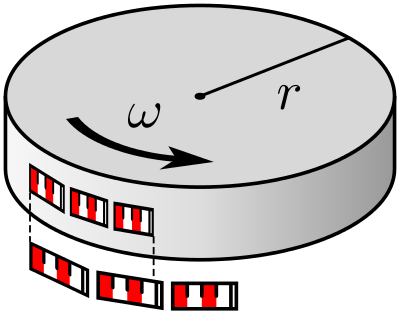
\includegraphics[height=80pt]{assets/Ehrenfest-paradox-disk.png}
    \captionof{figure}{Ehrenfest
    paradox disk}
\end{center}

However, since the radius is perpendicular to the direction of motion,
it will not undergo any contraction. So
\[\frac{\mathrm{circumference}}{\mathrm{diameter}}=\frac{2\pi R \sqrt{1-(\omega R)^2/c^2}}{2R} = \pi \sqrt{1-(\omega R)^2/c^2}.\]
This is paradoxical, since in accordance with Euclidean geometry, it
should be exactly equal to \(\pi\).
\end{quote}

The description above is taken from \emph{Wikipedia: Ehrenfest paradox}\newline (\url{https://en.wikipedia.org/w/index.php?title=Ehrenfest_paradox&oldid=1182372365}).

We can use another metric (张量) to analyze the Ehrenfest paradox. The
metric is
\[\mathrm{d}s^2 = \mathrm{d}r^2 + r^2 \mathrm{d}\theta^2 - c^2 \mathrm{d}t^2.\]

Substitute the relationship between reference frames \(S\) and \(S'\)
\[\left\{
    \begin{array}{l}
        r' = r, \\
        \theta' = \theta - \omega t, \\
        t' = t
    \end{array}
\right.\] in, and we get \begin{align*}
    \mathrm{d}s^2 & = \mathrm{d}r'^2 + r'^2 \left( \mathrm{d}\theta' + \omega \mathrm{d}t \right)^2 - c^2 \mathrm{d}t'^2 \\
    & = \mathrm{d}r'^2 + r'^2 \mathrm{d}\theta'^2 + 2 \omega r'^2 \mathrm{d}\theta' \mathrm{d}t - c^2 \left( 1 - \frac{r'^2 \omega^2}{c^2} \right) \mathrm{d}t'^2.
\end{align*}

Write this in tensor form, and we get
\[\mathrm{d} s^2 = g_{\mu\nu} \mathrm{d}x^{\mu} \mathrm{d}x^{\nu},\]
where \[\mathbf{g} = (g_{\mu\nu}) = \begin{pmatrix}
    1 & 0 & 0 \\
    0 & r'^2 & 2 \omega r'^2 \\
    0 & 0 & - c^2 \left( 1 - \dfrac{r'^2 \omega^2}{c^2} \right)
\end{pmatrix}.\]

\subsection*{(5) Minkowski spacetime
闵可夫斯基时空}\label{minkowski-spacetime-ux95f5ux53efux592bux65afux57faux65f6ux7a7a-2}

In Minkowski spacetime, we express a point within it in this form:
\[\boldsymbol{r} = (ct, x, y, z).\] This is an expression of the world
line (世界线), which is the path that an object traces in 4-dimensional
spacetime.

From \(\boldsymbol{r}\) we can calculate its velocity
\[\boldsymbol{v} = \frac{\mathrm{d} \boldsymbol{r}}{\mathrm{d} \tau} = \frac{\mathrm{d} \boldsymbol{r}}{\mathrm{d}t} \frac{\mathrm{d}t}{\mathrm{d} \tau} = \gamma \frac{\mathrm{d} \boldsymbol{r}}{\mathrm{d}t} = \gamma (c, \dot{x}, \dot{y}, \dot{z}),\]
and thus acceleration \begin{align*}
    \boldsymbol{a} & = \frac{\mathrm{d} \boldsymbol{v}}{\mathrm{d} \tau} = \frac{\mathrm{d} \boldsymbol{v}}{\mathrm{d}t} \frac{\mathrm{d}t}{\mathrm{d} \tau} = \gamma \frac{\mathrm{d} \boldsymbol{v}}{\mathrm{d}t} \\
    & = \gamma \frac{\mathrm{d}}{\mathrm{d}t} \Big[ \gamma \left( c, \dot{x}, \dot{y}, \dot{z} \right) \Big] \\
    & = \gamma \left[ \gamma (0, \ddot{x}, \ddot{y}, \ddot{z}) + \left( c, \dot{x}, \dot{y}, \dot{z} \right) \frac{\mathrm{d} \gamma}{\mathrm{d}t} \right].
\end{align*}

Here, \begin{align*}
    \frac{\mathrm{d} \gamma}{\mathrm{d}t} & = \frac{\mathrm{d}}{\mathrm{d}t} \left( 1 - \frac{\dot{x}^2 + \dot{y}^2 + \dot{z}^2}{c^2} \right)^{- 1/2} \\
    & = - \frac{1}{2} \left( 1 - \frac{\dot{x}^2 + \dot{y}^2 + \dot{z}^2}{c^2} \right)^{- 3/2} \left( - \frac{2 \dot{x} \ddot{x} + 2 \dot{y} \ddot{y} + 2 \dot{z} \ddot{z}}{c^2} \right) \\
    & = \frac{\dot{x} \ddot{x} + \dot{y} \ddot{y} + \dot{z} \ddot{z}}{c^2} \gamma^3.
\end{align*}

Substitute \(\displaystyle \frac{\mathrm{d} \gamma}{\mathrm{d}t}\) into
acceleration, and we acquire \begin{align*}
    \boldsymbol{a} ={} & \gamma^2 (0, \ddot{x}, \ddot{y}, \ddot{z}) + \left( c, \dot{x}, \dot{y}, \dot{z} \right)\frac{\dot{x} \ddot{x} + \dot{y} \ddot{y} + \dot{z} \ddot{z}}{c^2} \gamma^4 \\
    ={} & \biggl(  \frac{\dot{x} \ddot{x} + \dot{y} \ddot{y} + \dot{z} \ddot{z}}{c} \gamma^4, \gamma^2 \ddot{x} + \frac{\dot{x} \ddot{x} + \dot{y} \ddot{y} + \dot{z} \ddot{z}}{c^2} \gamma^4 \dot{x}, \\
    & \gamma^2 \ddot{y} + \frac{\dot{x} \ddot{x} + \dot{y} \ddot{y} + \dot{z} \ddot{z}}{c^2} \gamma^4 \dot{y}, \gamma^2 \ddot{z} + \frac{\dot{x} \ddot{x} + \dot{y} \ddot{y} + \dot{z} \ddot{z}}{c^2} \gamma^4 \dot{z} \biggr).
\end{align*}

From this, we can get 4-dimensional force \begin{align*}
    \boldsymbol{F} = m \boldsymbol{a} = m & \biggl(  \frac{\dot{x} \ddot{x} + \dot{y} \ddot{y} + \dot{z} \ddot{z}}{c} \gamma^4, \gamma^2 \ddot{x} + \frac{\dot{x} \ddot{x} + \dot{y} \ddot{y} + \dot{z} \ddot{z}}{c^2} \gamma^4 \dot{x}, \\
    & \gamma^2 \ddot{y} + \frac{\dot{x} \ddot{x} + \dot{y} \ddot{y} + \dot{z} \ddot{z}}{c^2} \gamma^4 \dot{y}, \gamma^2 \ddot{z} + \frac{\dot{x} \ddot{x} + \dot{y} \ddot{y} + \dot{z} \ddot{z}}{c^2} \gamma^4 \dot{z} \biggr).
\end{align*}

\subsection*{(6) Deduction of relativistic Lagrangian
相对论拉格朗日量的推导}\label{deduction-of-relativistic-lagrangian-ux76f8ux5bf9ux8bbaux62c9ux683cux6717ux65e5ux91cfux7684ux63a8ux5bfc}

Generalized momentum is
\[p = m \frac{\mathrm{d} \boldsymbol{q}}{\mathrm{d} \tau} = \gamma m \dot{q} = \frac{m \dot{q}}{\sqrt{1 - \dot{q}^2 / c^2}}. \quad(1)\]

By definition we know that
\[p \equiv \frac{\partial L}{\partial \dot{q}}.\]

Considering that: (a) \(L = T - V\), (b) \(V(q_1, q_2, \dots, q_s)\)
does not depend on \(\dot{q}_j\) and (c)
\(T(\dot{q}_1, \dot{q}_2, \dots, \dot{q}_s)\) does not depend on
\(q_j\), we can say that
\[p \equiv \frac{\partial \left( L + V \right)}{\partial \dot{q}} = \frac{\partial T}{\partial \dot{q}} = \frac{\mathrm{d} T}{\mathrm{d} \dot{q}}. \quad(2)\]

From \((1)\) and \((2)\), we can acquire an equation for Lagrangian
\(L\):
\[\frac{\mathrm{d} T}{\mathrm{d} \dot{q}} = \frac{m \dot{q}}{\sqrt{1 - \dot{q}^2 / c^2}}.\]

Solve this:
\[\mathrm{d} T = \frac{m \dot{q} \mathrm{d} \dot{q}}{\sqrt{1 - \dot{q}^2 / c^2}} = \frac{m \mathrm{d}\left( \dot{q}^2 \right)}{2 \sqrt{1 - \dot{q}^2 / c^2}} = - \frac{1}{2} mc^2 \mathrm{d} \left( 2 \sqrt{1 - \frac{\dot{q}^2}{c^2}} \right) = - mc^2 \mathrm{d} \sqrt{1 - \frac{\dot{q}^2}{c^2}}.\]

Integrate this, we can get
\[T = - mc^2 \sqrt{1 - \frac{\dot{q}^2}{c^2}}.\]

Thus the Lagrangian
\[L = T - V = - mc^2 \sqrt{1 - \frac{\dot{q}^2}{c^2}} - V.\]

\begin{quote}
作业:推导 \(H = \gamma mc^2 + V\).

答案:\begin{align*}
H & = p \dot{q} - L \\
& = \frac{m \dot{q}}{\sqrt{1 - \dot{q}^2 / c^2}} \dot{q} - \left( - mc^2 \sqrt{1 - \frac{\dot{q}^2}{c^2}} - V \right) \\
& = \frac{m \dot{q}^2}{\sqrt{1 - \dot{q}^2 / c^2}} + \frac{mc^2 \left( 1 - \dfrac{\dot{q}^2}{c^2} \right)}{\sqrt{1 - \dot{q}^2 / c^2}} + V \\
& = \frac{m c^2}{\sqrt{1 - \dot{q}^2 / c^2}} + V \\
& = \gamma mc^2 + V.
\end{align*}
\end{quote}
